\documentclass{beamer}

\usepackage[utf8]{inputenc}
\usecolortheme{beaver}
\usepackage{caption}
\usepackage{subcaption}
\usepackage{mathtools}
\usepackage{todonotes}
\usepackage{amsmath}
\usepackage{bm}
\usepackage{listings}
\usepackage{ragged2e}
\usepackage{titlecaps}
\usepackage{fancyvrb}

\def\ci{\perp\!\!\!\!\!\perp}

\newtheorem{proposition}{Proposition}
\Addlcwords{for a is but and with of in as the etc on to if}

\setbeamertemplate{section in toc}{\inserttocsectionnumber.~\inserttocsection}
\usetheme{Boadilla}
\makeatletter
\setbeamertemplate{footline}{%
    \leavevmode%
    \hbox{%
        \begin{beamercolorbox}[wd=.3\paperwidth,ht=2.25ex,dp=1ex,center]{author in head/foot}%
            \usebeamerfont{author in head/foot}\insertshortauthor\expandafter\beamer@ifempty\expandafter{\beamer@shortinstitute}{}{~~(\insertshortinstitute)}
        \end{beamercolorbox}%
        \begin{beamercolorbox}[wd=.55\paperwidth,ht=2.25ex,dp=1ex,center]{title in head/foot}%
            \usebeamerfont{title in head/foot}\insertshorttitle
        \end{beamercolorbox}%
        \begin{beamercolorbox}[wd=.15\paperwidth,ht=2.25ex,dp=1ex,right]{date in head/foot}%
            \usebeamerfont{date in head/foot}\insertshortdate{}\hspace*{2em} \insertframenumber{} / \inserttotalframenumber\hspace*{2ex} 
        \end{beamercolorbox}}%
        \vskip0pt%
    }
\makeatother

\begin{document}

\title[]{Self-Compatibility: Evaluating Causal Discovery without Ground Truth}
\date{}

\begin{frame}
	\begin{figure}
		\centering
		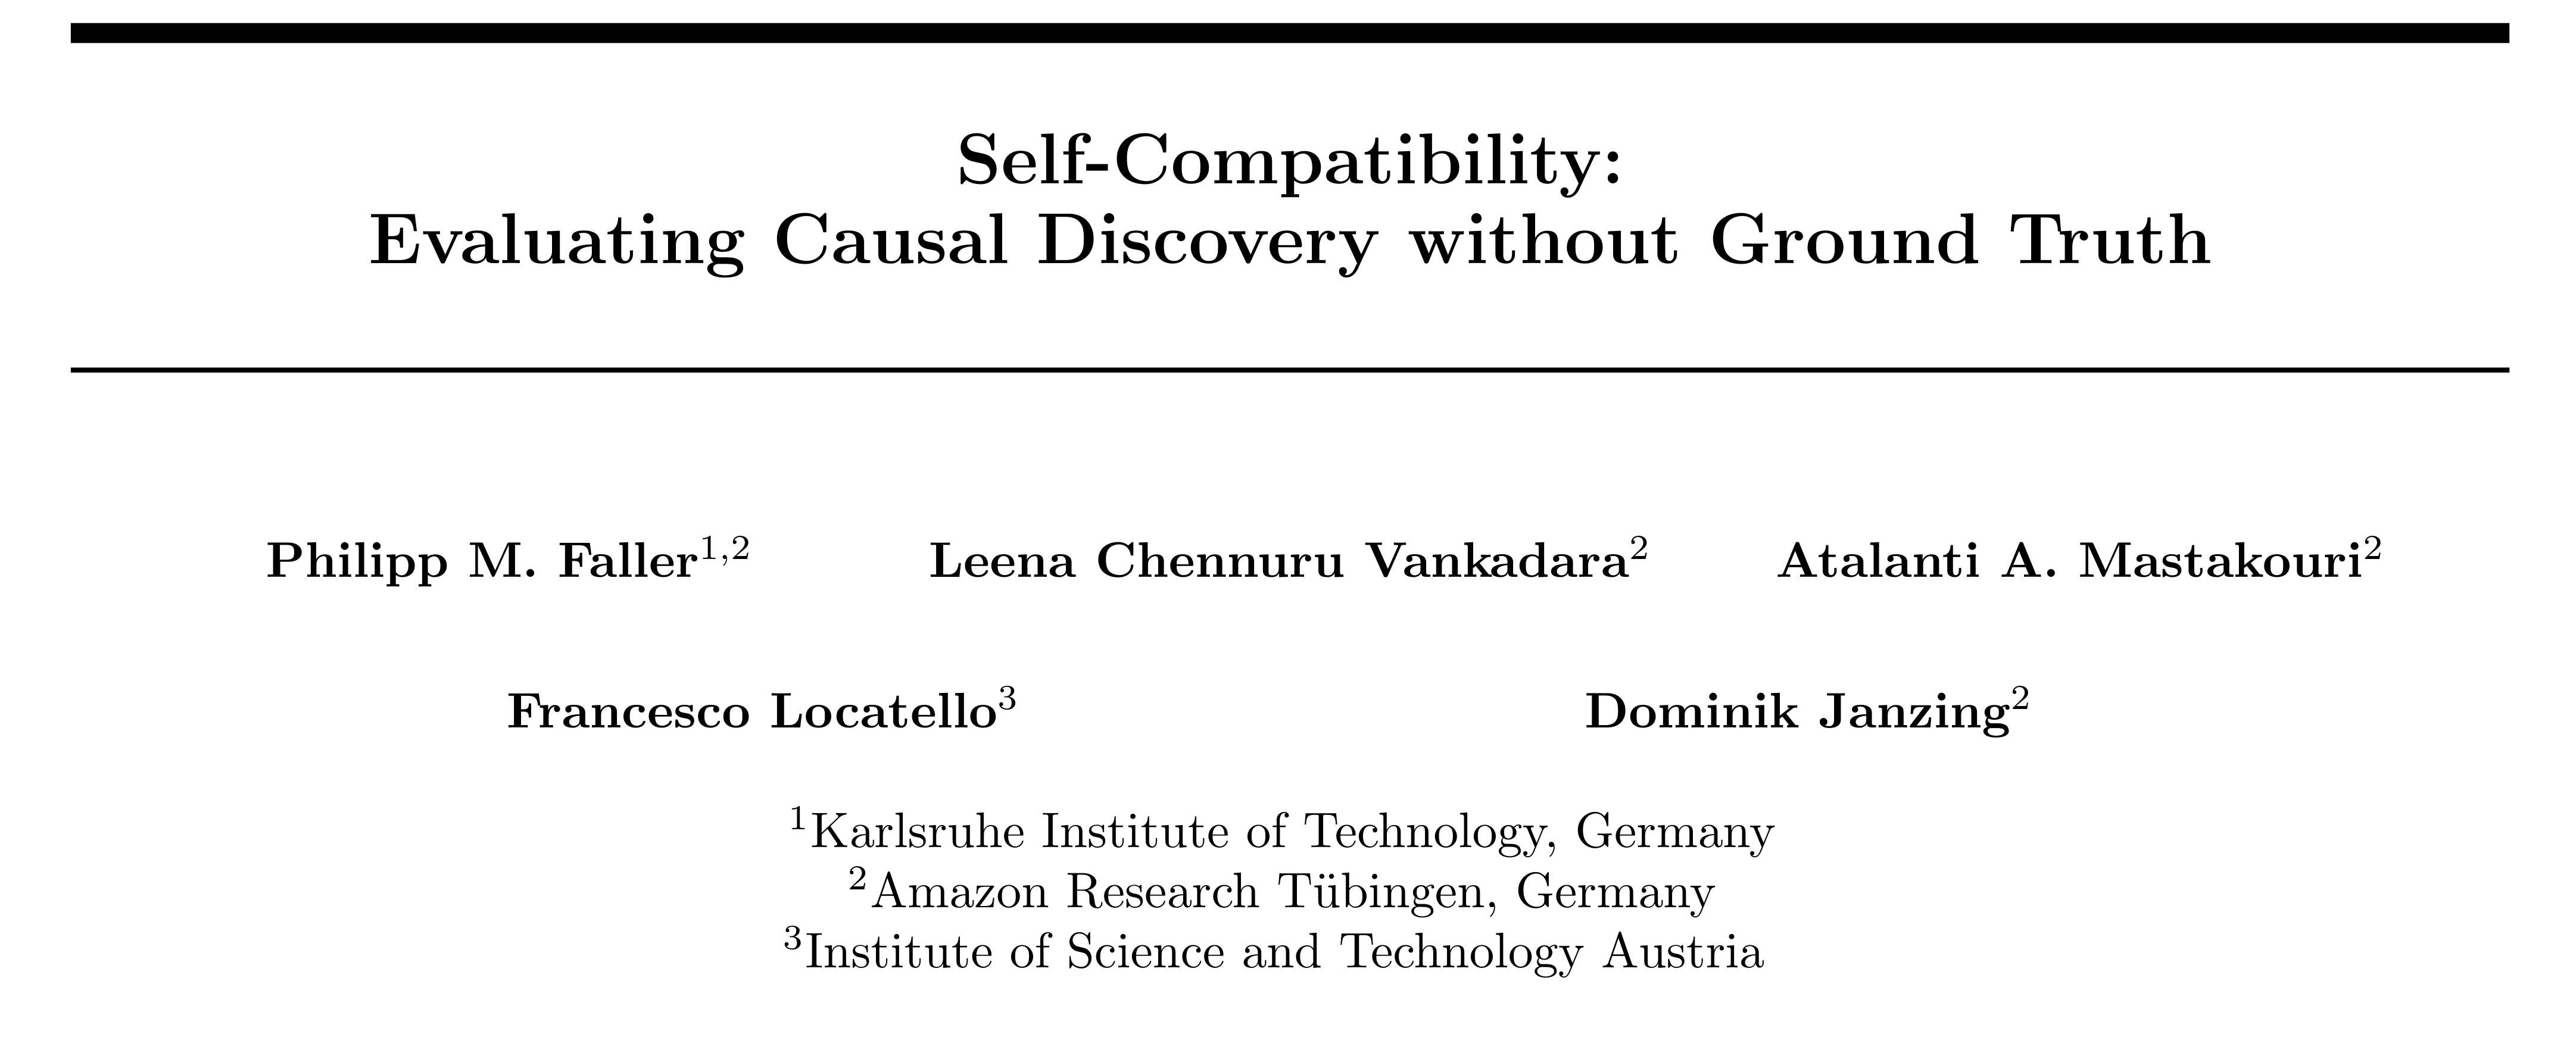
\includegraphics[scale=0.08]{imgs/title.png}
	\end{figure}
\end{frame}

\begin{frame}{Directed Acyclic Graphs (DAGs)}
	\begin{columns}
		\begin{column}{0.55\textwidth}
		\begin{itemize}
			\item Nodes represent random variables.
			\item Edges represent causal relationships.
			\item E.g., \textbf{Education} has a direct effect on \textbf{Income}. 
			\item E.g., \textbf{Age} has indirect effect on \textbf{Income} through \textbf{Education} and \textbf{Hours Per Week}.
			\item Used for causal effect estimation.
		\end{itemize}
		\end{column}

		\begin{column}{0.45 \textwidth}
		\begin{figure}
			\centering
			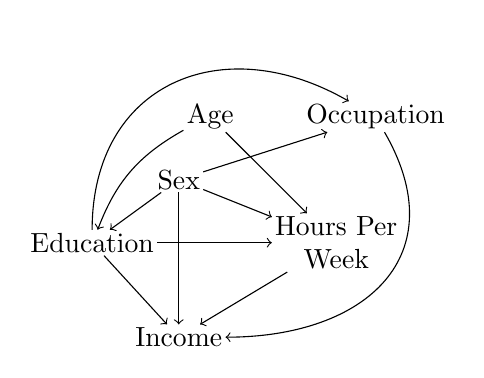
\begin{tikzpicture}[scale=1]
			\tikzstyle{every node}=[align=center, inner sep=1pt]
				\node (sex) at (-0.7, -0.8) {Sex};
				\node (age) at (-0.3, 0) {Age};
				\node (ed) at (-1.8, -1.6) {Education};
				\node (occ) at (1.8, 0) {Occupation};
				\node (hrpw) at (1.3, -1.6) {Hours Per \\ Week};
				\node (income) at (-0.7, -2.8) {Income};
			
				\draw[->]  (age) to[bend right=20] (ed);
				\draw[->]  (sex) to (ed);
				\draw[->]  (age) to (hrpw);
				\draw[->]  (ed) to (hrpw);
				\draw[->]  (sex) to (hrpw);
				\draw[->]  (ed) to (income);
				\draw[->]  (hrpw) to (income);
				\draw[->]  (occ) to[out=300, in=0, looseness=1.4] (income.east);
				\draw[->]  (sex) to (income);
				\draw[->]  (ed) to[out=90, in=150, looseness=1.3] (occ);
				\draw[->]  (sex) to (occ);	
			\end{tikzpicture}
			\caption*{\footnotesize {Example of a Causal Model / DAG}}
		\end{figure}
		\end{column}
	\end{columns}	
\end{frame}

% \begin{frame}{Interventions on DAGs}
% 	\begin{itemize}
% 		\item DAGs allow interventions that can be used to estimate causal effect. 
% 		\item For example, we can intervene on Hours
% 	\end{itemize}
% \end{frame}

\begin{frame}{DAGs and Data}
	\begin{itemize}
		\item DAGs and Data are connected through faithfulness assumption.
		\item Every implied conditional independence (CI) statement hold in the data.
		\item Every CI in data holds in the DAG.
	\end{itemize}
	\begin{figure}
		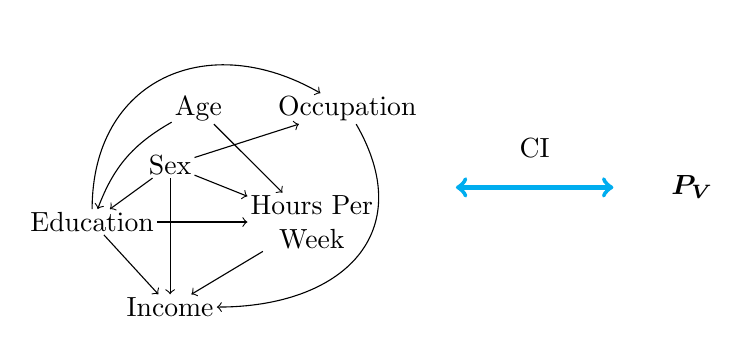
\begin{tikzpicture}
			\begin{scope}[scale=0.9]
			\tikzstyle{every node}=[align=center, inner sep=1pt]
				\node (sex) at (-0.7, -0.8) {Sex};
				\node (age) at (-0.3, 0) {Age};
				\node (ed) at (-1.8, -1.6) {Education};
				\node (occ) at (1.8, 0) {Occupation};
				\node (hrpw) at (1.3, -1.6) {Hours Per \\ Week};
				\node (income) at (-0.7, -2.8) {Income};
			
				\draw[->]  (age) to[bend right=20] (ed);
				\draw[->]  (sex) to (ed);
				\draw[->]  (age) to (hrpw);
				\draw[->]  (ed) to (hrpw);
				\draw[->]  (sex) to (hrpw);
				\draw[->]  (ed) to (income);
				\draw[->]  (hrpw) to (income);
				\draw[->]  (occ) to[out=300, in=0, looseness=1.4] (income.east);
				\draw[->]  (sex) to (income);
				\draw[->]  (ed) to[out=90, in=150, looseness=1.3] (occ);
				\draw[->]  (sex) to (occ);	
			\end{scope}
			\begin{scope}[xshift=3cm, yshift=-1cm]
				\node(ci) at (1, 0.5) {CI};
				\draw[ultra thick,<->,cyan] (0,0) -- (2,0);
			\end{scope}
			\begin{scope}[xshift=6cm, yshift=-1cm]
				\node(dist) at ( 0, 0) {$ \bm{P}_{\bm{V}} $};
			\end{scope}
		\end{tikzpicture}
	\end{figure}
	
\end{frame}

\begin{frame}{Causal Discovery: Learning DAGs From Data}
	\vspace{-2em}
	\begin{figure}
		\centering
		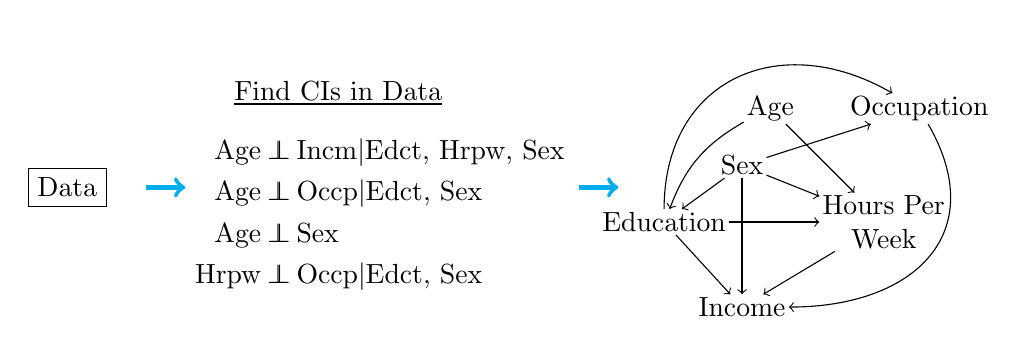
\begin{tikzpicture}
			\node[draw, rectangle] (data) at (0, 0) {Data};
			\draw[ultra thick,->, cyan] (1,0) -- (1.5,0);
			\node[rectangle, align=center, inner sep=1pt] at (3.5, 0) {
				\begin{minipage}{0.3\textwidth}
					\center{\underline{\textnormal{Find CIs in Data}}}
					\begin{equation*}
						\begin{split}
							\textnormal{Age} &\ci \textnormal{Incm} \rvert \textnormal{Edct, Hrpw, Sex} \\
							\textnormal{Age} &\ci \textnormal{Occp} \rvert \textnormal{Edct, Sex} \\
							\textnormal{Age} &\ci \textnormal{Sex} \\
							\textnormal{Hrpw} &\ci \textnormal{Occp} \rvert \textnormal{Edct, Sex} \\
						\end{split}
					\end{equation*}
				\end{minipage}
				};
			\begin{scope}[xshift=6.5cm]
				\draw[ultra thick,->,cyan] (0,0) -- (0.5,0);
			\end{scope}	
			\begin{scope}[xshift=9.2cm, yshift=1cm, scale=0.9]
				\tikzstyle{every node}=[align=center, inner sep=1pt]
				\node (sex) at (-0.7, -0.8) {Sex};
				\node (age) at (-0.3, 0) {Age};
				\node (ed) at (-1.8, -1.6) {Education};
				\node (occ) at (1.8, 0) {Occupation};
				\node (hrpw) at (1.3, -1.6) {Hours Per \\ Week};
				\node (income) at (-0.7, -2.8) {Income};

				\draw[->]  (age) to[bend right=20] (ed);
				\draw[->]  (sex) to (ed);
				\draw[->]  (age) to (hrpw);
				\draw[->]  (ed) to (hrpw);
				\draw[->]  (sex) to (hrpw);
				\draw[->]  (ed) to (income);
				\draw[->]  (hrpw) to (income);
				\draw[->]  (occ) to[out=300, in=0, looseness=1.4] (income.east);
				\draw[->]  (sex) to (income);
				\draw[->]  (ed) to[out=90, in=150, looseness=1.3] (occ);
				\draw[->]  (sex) to (occ);
			\end{scope}
		\end{tikzpicture}
	\end{figure}
	\vspace{2em}
	\center{\textcolor{red}{Unsupervised learning problem}: No ground truth DAG.}
\end{frame}

\begin{frame}{Problems with Causal Discovery}
	\begin{figure}
		\centering
		\begin{subfigure}{\textwidth}
			\centering
			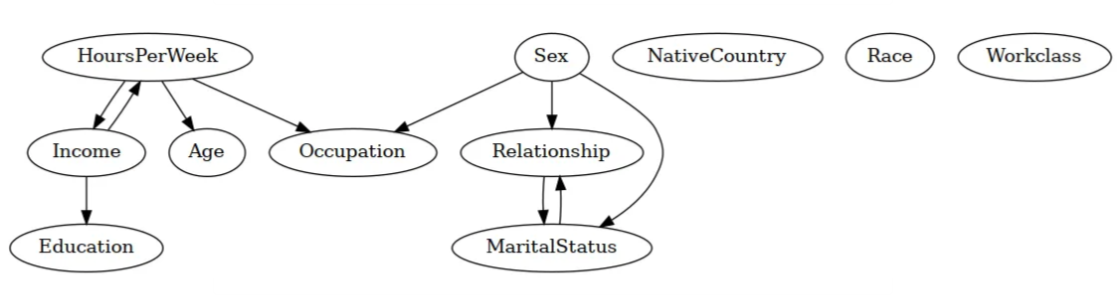
\includegraphics[scale=0.25]{imgs/pdag_pc.png}
			\caption{PC algorithm}
		\end{subfigure}
		\begin{subfigure}{\textwidth}
			\centering
			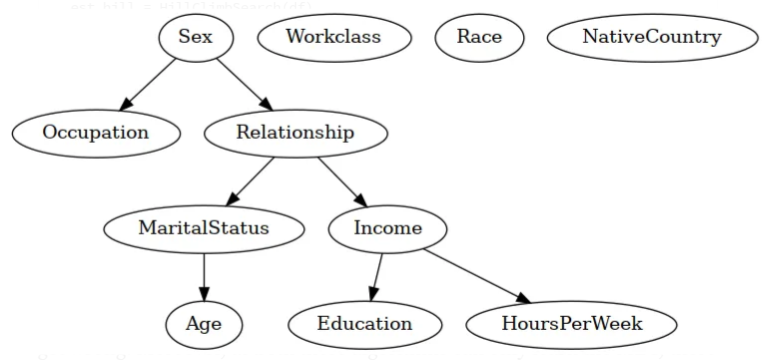
\includegraphics[scale=0.25]{imgs/pdag_hill.png}
			\caption{Hill-Climb Search Algorithm}
		\end{subfigure}
	\end{figure}
\end{frame}

\begin{frame}{Problems with Causal Discovery}
	\begin{figure}
		\centering
		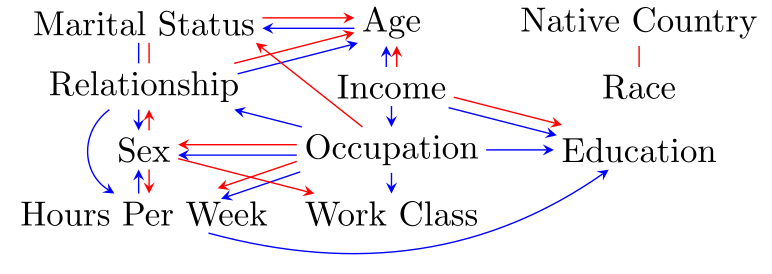
\includegraphics[scale=0.3]{imgs/pc_sample.png}
		\caption{PC algorithm with residualization based test. Red N=400, Blue N=800}
	\end{figure}
\end{frame}

\begin{frame}{Problems with Causal Discovery}
	\begin{itemize}
		\item Casual discovery algorithms make assumptions that might not be satisfied in the data.
		\item Finite samples can lead to errors.
	\end{itemize}
\end{frame}

\begin{frame}{Problem Statement}
	\center{Given a dataset, how to evaluate the performance of a causal discovery algorithm?}
\end{frame}

\begin{frame}{Self-compatibility: Idea}
	\begin{figure}
		\centering
		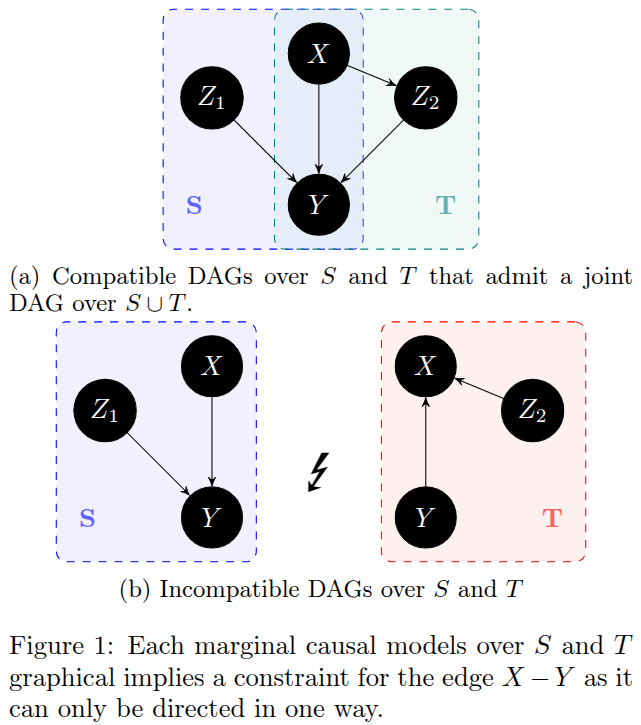
\includegraphics[scale=0.3]{imgs/example.png}
	\end{figure}
\end{frame}

\begin{frame}{Interventional Compatibility}
	\begin{figure}
		\centering
		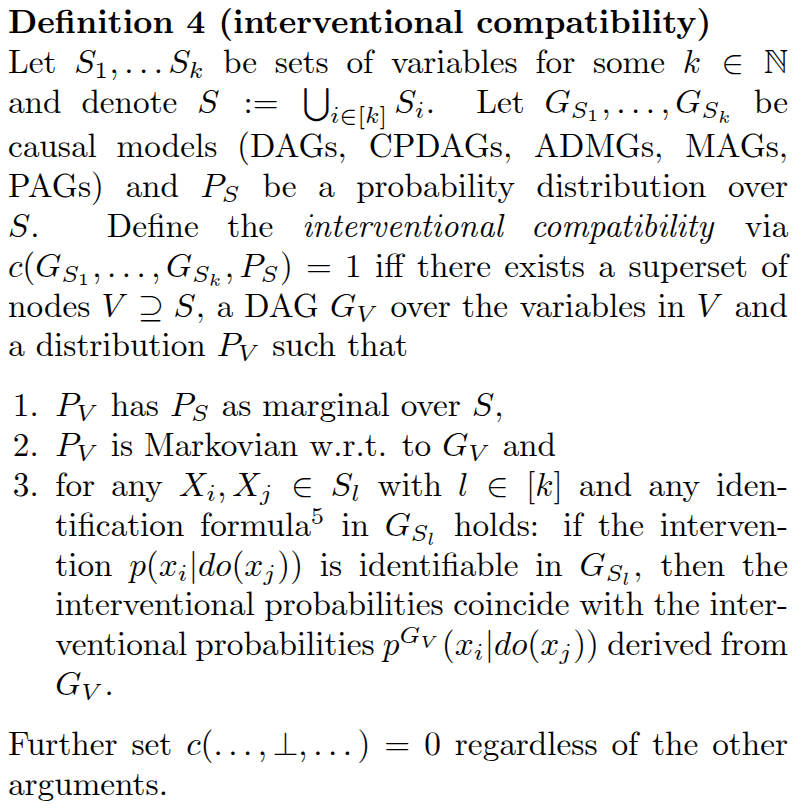
\includegraphics[scale=0.25]{imgs/def4.png}
	\end{figure}
\end{frame}

\begin{frame}{Interventional Compatibility: Example}
	\begin{figure}
		\centering
		\begin{subfigure}{0.3 \textwidth}
			\centering
			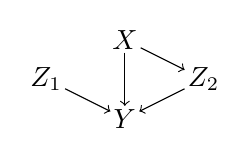
\begin{tikzpicture}
				\tikzstyle{every node}=[align=center, inner sep=1pt]\
				\node (X) at (0, 0) {$ X $};
				\node (Y) at (0, -1) {$ Y $};
				\node (Z1) at (-1, -0.5) {$ Z_1 $};
				\node (Z2) at (1, -0.5) {$ Z_2 $};

				\draw[->]  (X) to (Y);
				\draw[->]  (X) to (Z2);
				\draw[->]  (Z1) to (Y);
				\draw[->]  (Z2) to (Y);
			\end{tikzpicture}
			\caption*{True DAG: $ V = S = \{ X, Y, Z_1, Z_2 \} $}
		\end{subfigure}
		\begin{subfigure}{0.3 \textwidth}
			\centering
			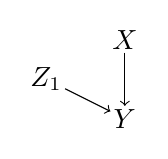
\begin{tikzpicture}
				\tikzstyle{every node}=[align=center, inner sep=1pt]\
				\node (X) at (0, 0) {$ X $};
				\node (Y) at (0, -1) {$ Y $};
				\node (Z1) at (-1, -0.5) {$ Z_1 $};

				\draw[->]  (X) to (Y);
				\draw[->]  (Z1) to (Y);
			\end{tikzpicture}
			\caption*{$S_1 = \{X, Y, Z_1 \}$}
		\end{subfigure}
		\begin{subfigure}{0.3 \textwidth}
			\centering
			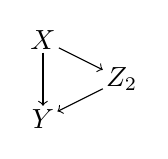
\begin{tikzpicture}
				\tikzstyle{every node}=[align=center, inner sep=1pt]\
				\node (X) at (0, 0) {$ X $};
				\node (Y) at (0, -1) {$ Y $};
				\node (Z2) at (1, -0.5) {$ Z_2 $};

				\draw[->]  (X) to (Y);
				\draw[->]  (X) to (Z2);
				\draw[->]  (Z2) to (Y);
			\end{tikzpicture}
			\caption*{$S_2 = \{ X, Y, Z_2 \} $}
		\end{subfigure}
	\end{figure}

	\begin{equation}
		\begin{split}
			\textnormal{True DAG}&: P(Y | do(X)) = \sum_{z \in Z_2} P(Y | X, Z_2=z) P(Z_2=z) \\
			S_1&: P(Y | do(X)) = P(Y | X) \\
			S_2&: P(Y | do(X)) = \sum_{z \in Z_2} P(Y | X, Z_2=z) P(Z_2=z) 
		\end{split}
	\end{equation}

	\vspace{0.5em}
	\center{$S_1$ and $S_2$ are not interventional compatible?}

\end{frame}

\begin{frame}{Graphical Compatibility: Latent ADMG}
	\begin{figure}
		\centering
		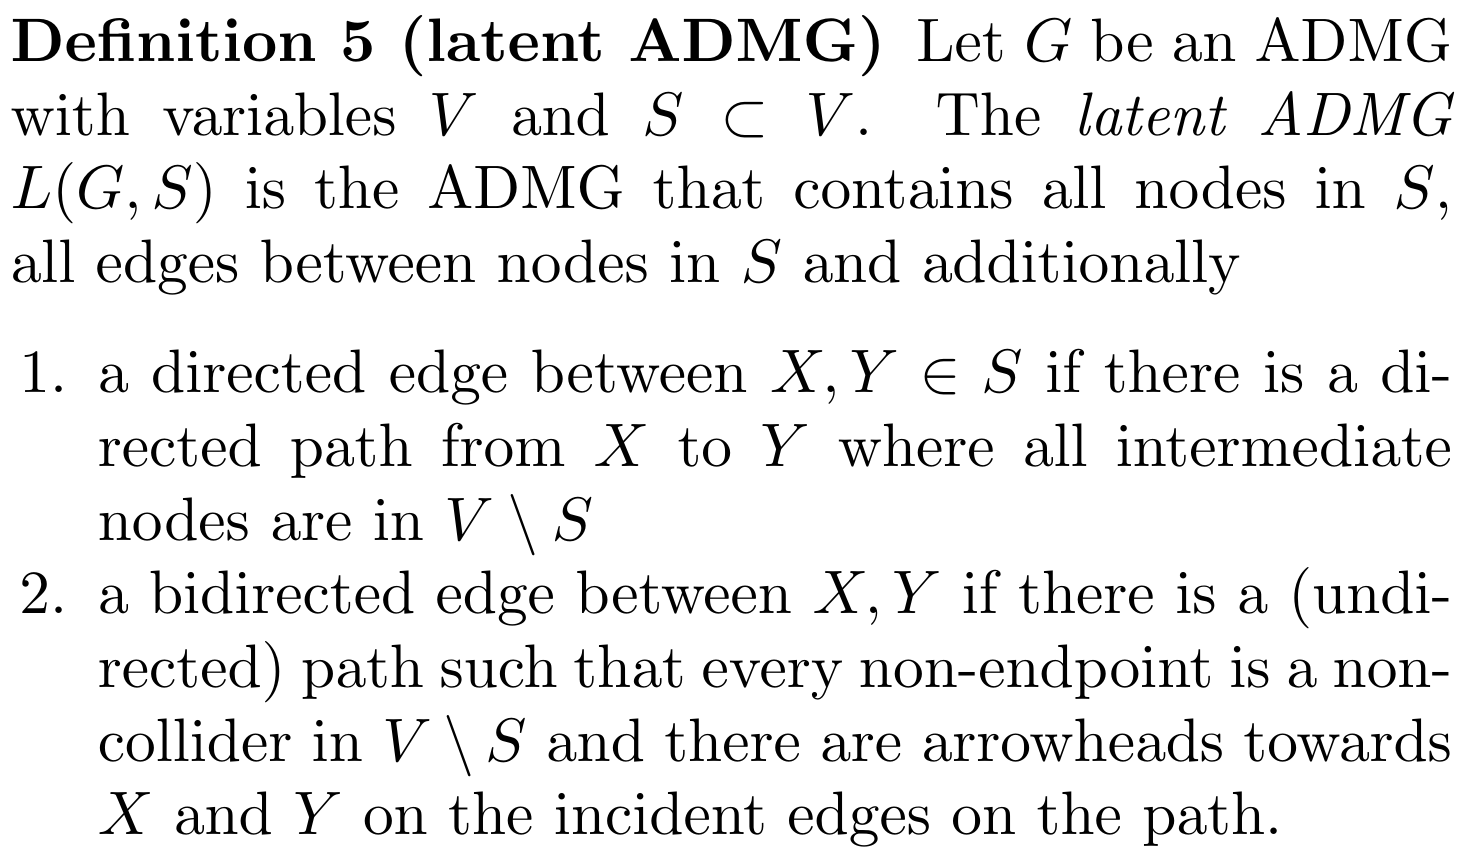
\includegraphics[scale=0.15]{imgs/def_5.png}
	\end{figure}
\end{frame}

\begin{frame}{Graphical Compatibility: Latent ADMG: Example}
	\begin{figure}
		\centering
		\begin{subfigure}{0.3 \textwidth}
			\centering
			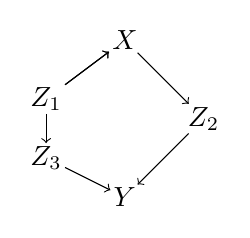
\begin{tikzpicture}
				\tikzstyle{every node}=[align=center, inner sep=1pt]\
				\node (X) at (0, 0) {$ X $};
				\node (Y) at (0, -2) {$ Y $};
				\node (Z1) at (-1, -1.5) {$ Z_3 $};
				\node (Z2) at (1, -1) {$ Z_2 $};
				\node (Z3) at (-1, -0.75) {$ Z_1 $};

				\draw[->]  (X) to (Z2);
				\draw[->]  (Z1) to (Y);
				\draw[->]  (Z2) to (Y);
				\draw[->]  (Z3) to (X);
				\draw[->]  (Z3) to (X);
				\draw[->]  (Z3) to (Z1);

			\end{tikzpicture}
			\caption*{True DAG}
		\end{subfigure}
		\begin{subfigure}{0.3 \textwidth}
			\centering
			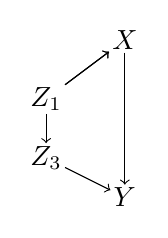
\begin{tikzpicture}
				\tikzstyle{every node}=[align=center, inner sep=1pt]\
				\node (X) at (0, 0) {$ X $};
				\node (Y) at (0, -2) {$ Y $};
				\node (Z1) at (-1, -1.5) {$ Z_3 $};
				\node (Z3) at (-1, -0.75) {$ Z_1 $};

				\draw[->]  (X) to (Y);
				\draw[->]  (Z1) to (Y);
				\draw[->]  (Z3) to (X);
				\draw[->]  (Z3) to (X);
				\draw[->]  (Z3) to (Z1);
			\end{tikzpicture}
			\caption*{Latent ADMG $S_1 = \{X, Y, Z_1, Z_3 \} $}
		\end{subfigure}
		\begin{subfigure}{0.3 \textwidth}
			\centering
			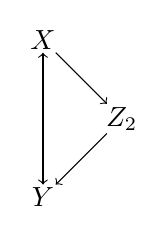
\begin{tikzpicture}
				\tikzstyle{every node}=[align=center, inner sep=1pt]\
				\node (X) at (0, 0) {$ X $};
				\node (Y) at (0, -2) {$ Y $};
				\node (Z2) at (1, -1) {$ Z_2 $};

				\draw[->]  (X) to (Z2);
				\draw[->]  (Z2) to (Y);
				\draw[<->] (X) to (Y);
			\end{tikzpicture}
			\caption*{Latent ADMG $S_2 = \{X, Y, Z_2\} $}
		\end{subfigure}

	\end{figure}
\end{frame}

\begin{frame}{Graphical Compatibility}
	\begin{figure}
		\centering
		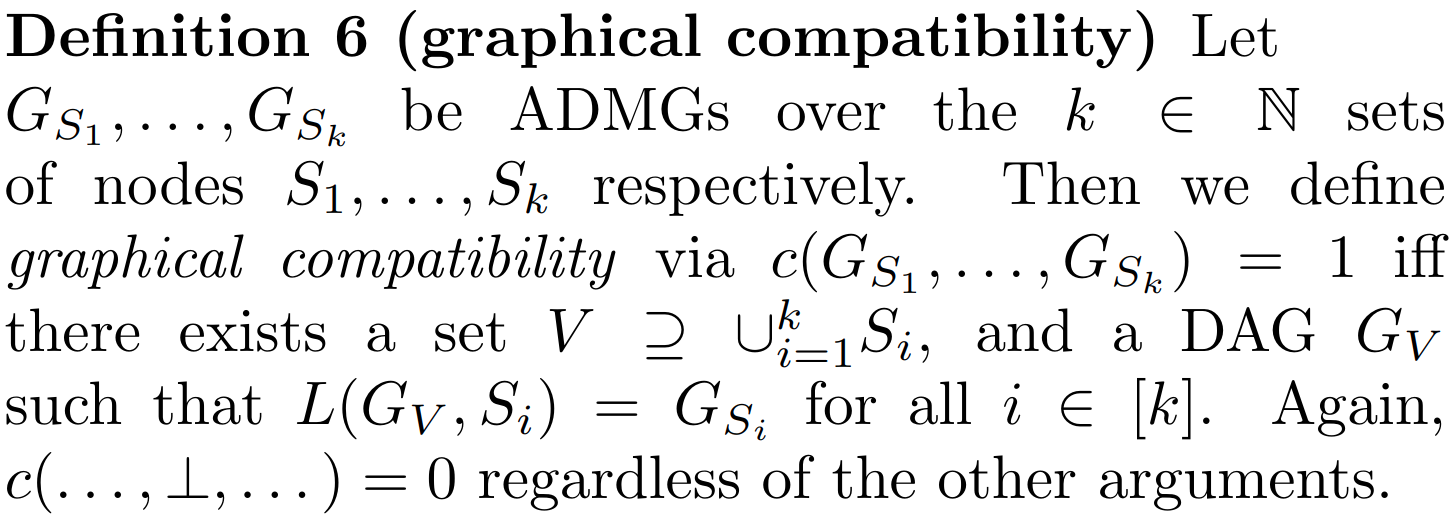
\includegraphics[scale=0.15]{imgs/def_6.png}
	\end{figure}
\end{frame}

\begin{frame}{Graphical Compatibility}
	\begin{figure}
		\centering
		\begin{subfigure}{0.3 \textwidth}
			\centering
			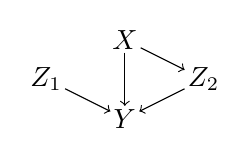
\begin{tikzpicture}
				\tikzstyle{every node}=[align=center, inner sep=1pt]\
				\node (X) at (0, 0) {$ X $};
				\node (Y) at (0, -1) {$ Y $};
				\node (Z1) at (-1, -0.5) {$ Z_1 $};
				\node (Z2) at (1, -0.5) {$ Z_2 $};

				\draw[->]  (X) to (Y);
				\draw[->]  (X) to (Z2);
				\draw[->]  (Z1) to (Y);
				\draw[->]  (Z2) to (Y);
			\end{tikzpicture}
			\caption*{True DAG: $ V = S = \{ X, Y, Z_1, Z_2 \} $}
		\end{subfigure}
		\begin{subfigure}{0.3 \textwidth}
			\centering
			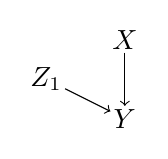
\begin{tikzpicture}
				\tikzstyle{every node}=[align=center, inner sep=1pt]\
				\node (X) at (0, 0) {$ X $};
				\node (Y) at (0, -1) {$ Y $};
				\node (Z1) at (-1, -0.5) {$ Z_1 $};

				\draw[->]  (X) to (Y);
				\draw[->]  (Z1) to (Y);
			\end{tikzpicture}
			\caption*{$S_1 = \{X, Y, Z_1 \}$}
		\end{subfigure}
		\begin{subfigure}{0.3 \textwidth}
			\centering
			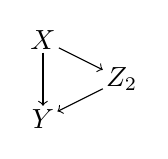
\begin{tikzpicture}
				\tikzstyle{every node}=[align=center, inner sep=1pt]\
				\node (X) at (0, 0) {$ X $};
				\node (Y) at (0, -1) {$ Y $};
				\node (Z2) at (1, -0.5) {$ Z_2 $};

				\draw[->]  (X) to (Y);
				\draw[->]  (X) to (Z2);
				\draw[->]  (Z2) to (Y);
			\end{tikzpicture}
			\caption*{$S_2 = \{ X, Y, Z_2 \} $}
		\end{subfigure}
	\end{figure}

	\vspace{0.5em}
	\center{$S_1$ and $S_2$ are graphically compatible.}
\end{frame}

\begin{frame}{Interventional Score}
	\begin{figure}
		\begin{subfigure}{\textwidth}
			\centering
			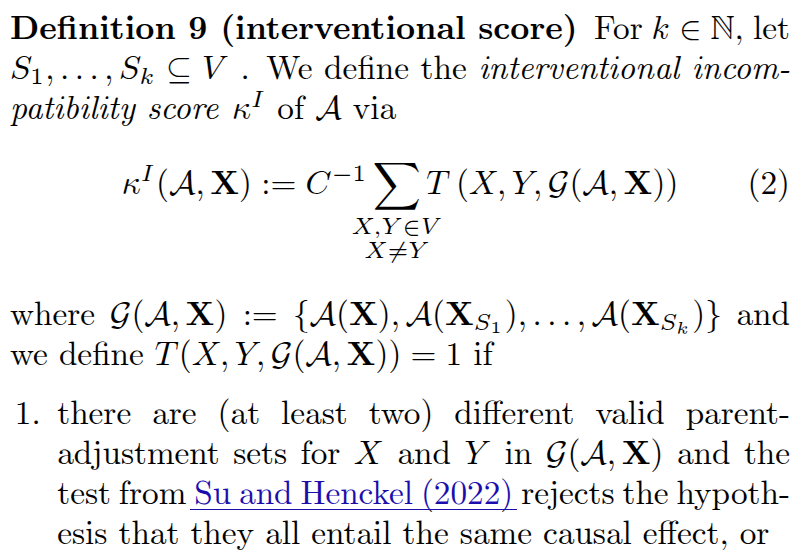
\includegraphics[scale=0.23]{imgs/def_9_1.png}
		\end{subfigure}
		\begin{subfigure}{\textwidth}
			\centering
			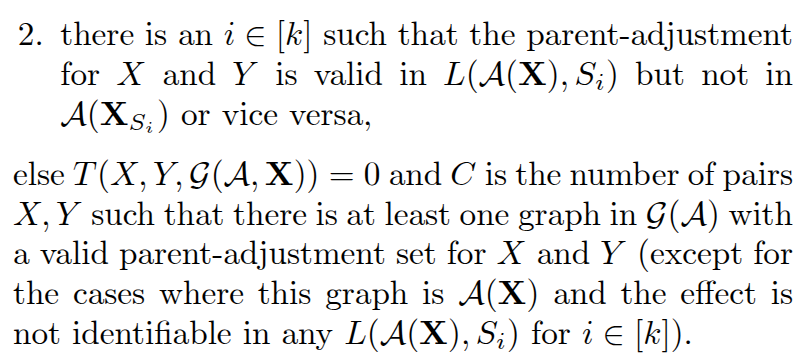
\includegraphics[scale=0.23]{imgs/def_9_2.png}
		\end{subfigure}
	\end{figure}
\end{frame}

\begin{frame}
	Add example
\end{frame}


\begin{frame}{Graphical Incompatibility Score}
	\begin{figure}
		\centering
		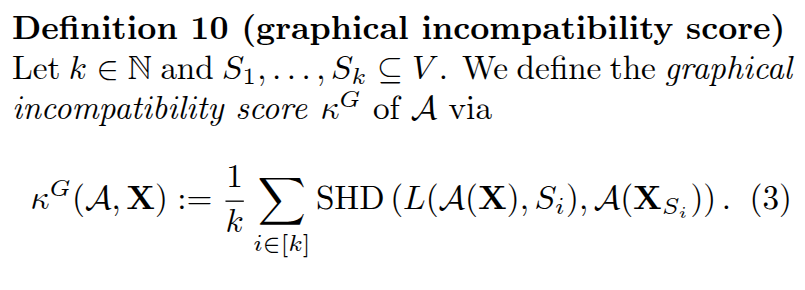
\includegraphics[scale=0.25]{imgs/def_10.png}
	\end{figure}
\end{frame}

\begin{frame}
	Add example
\end{frame}


\begin{frame}{Empirical Results}
	\begin{figure}
		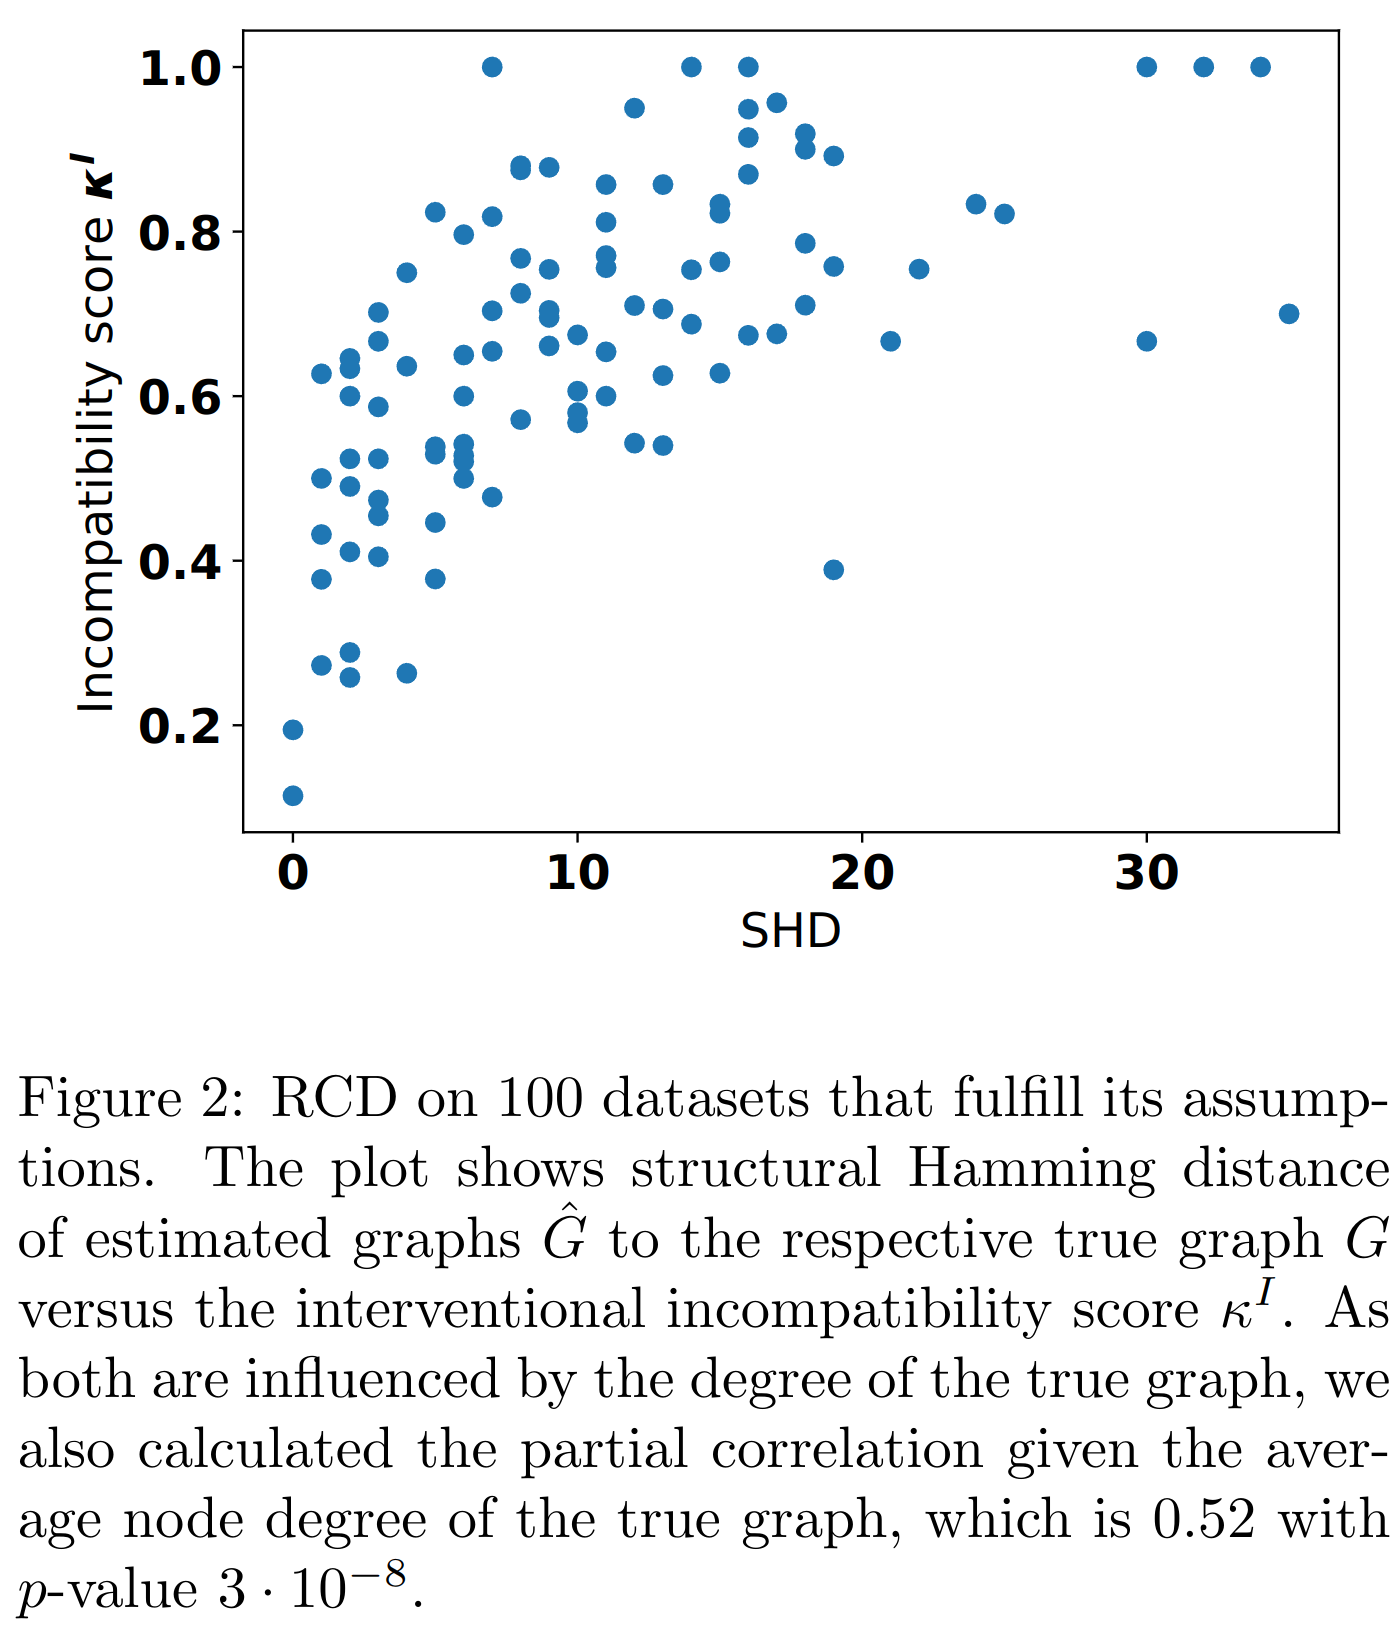
\includegraphics[scale=0.12]{imgs/empirical1.png}
	\end{figure}
\end{frame}

\begin{frame}{Empirical Results}
	\begin{figure}
		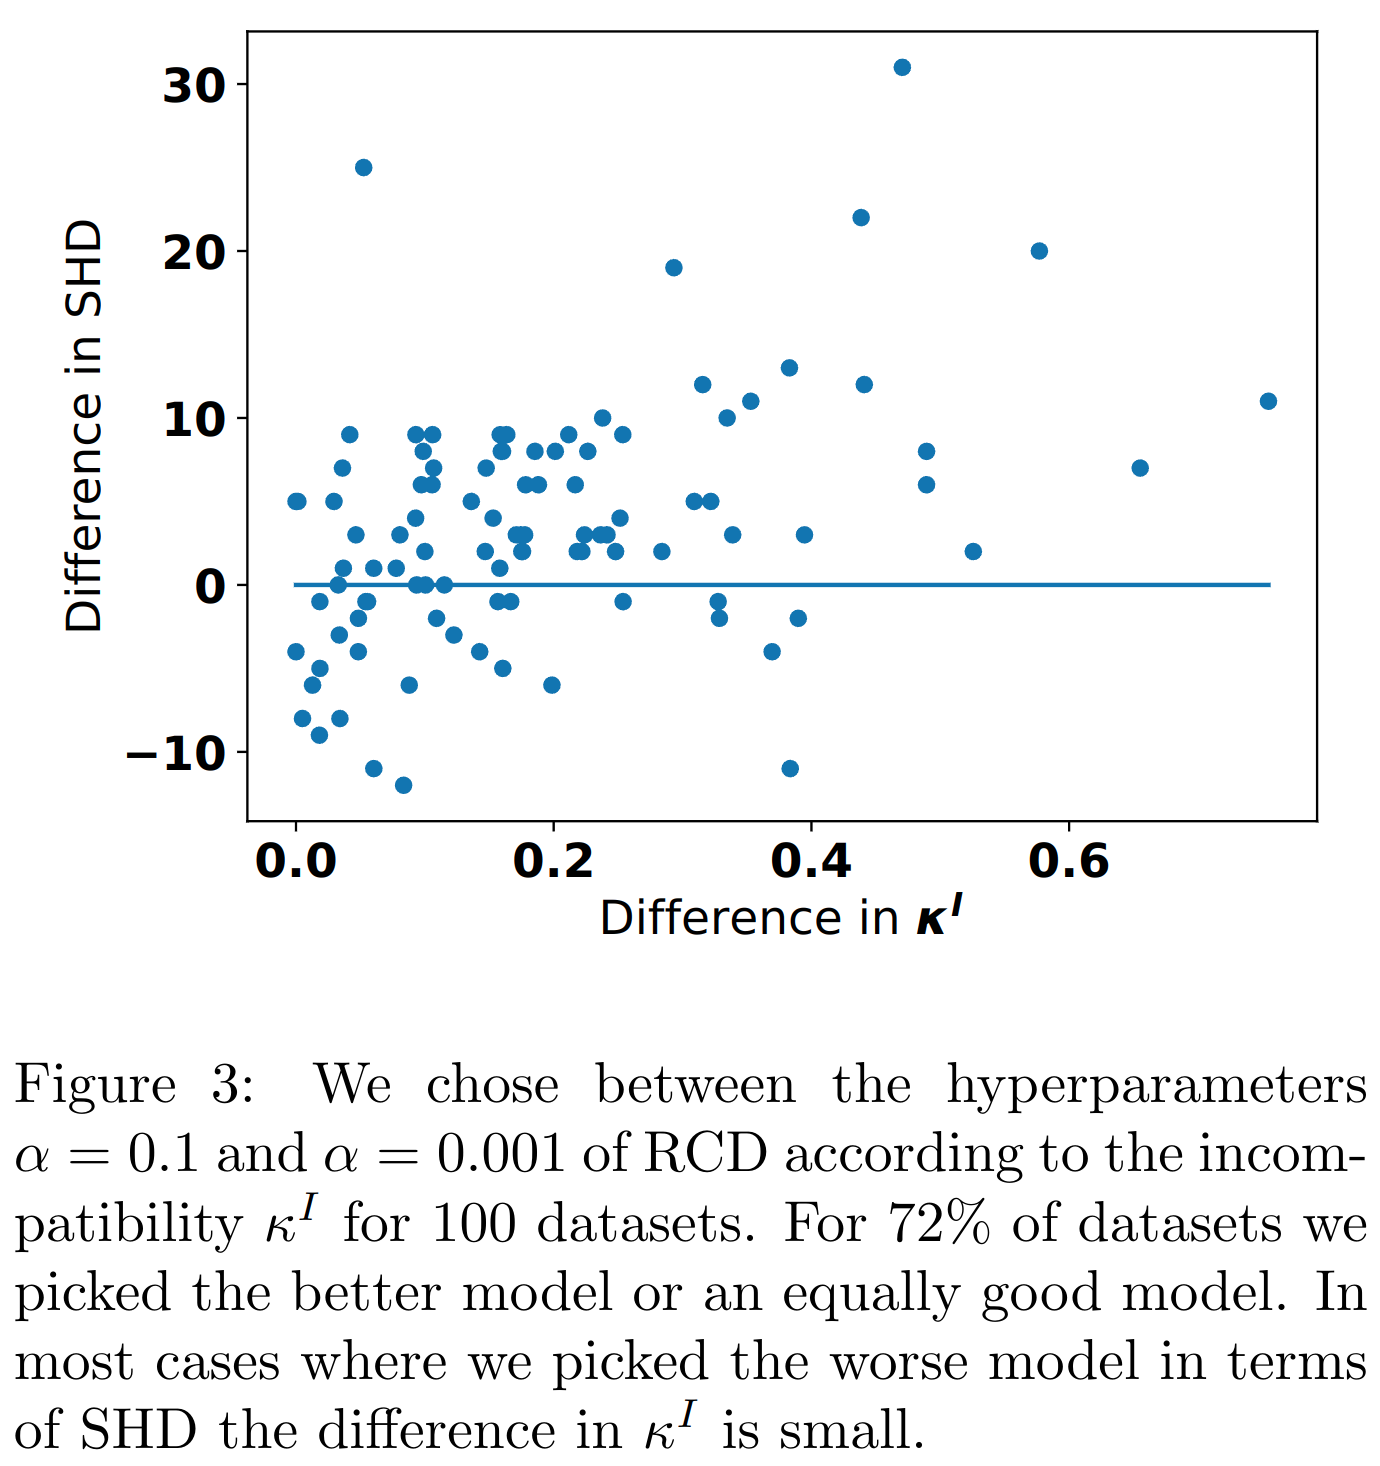
\includegraphics[scale=0.12]{imgs/empirical2.png}
	\end{figure}
\end{frame}

\begin{frame}{Conclusion}
	\begin{itemize}
		\item Method to falsify output of causal discovery algorithms in the absence of ground truth.
		\item Incompatibility score can be used as a proxy for SHD as shown empirically.
		\item However, no theoretical guarantees.
		\item What is an acceptable threshold for incompatibility score?
	\end{itemize}
\end{frame}

\end{document}
